\documentclass[letterpaper]{article}
\usepackage[submission]{aaai2027}
\usepackage[hyphens]{url}
\usepackage{graphicx}
\urlstyle{rm}
\def\UrlFont{\rm}
\usepackage{natbib}
\usepackage{caption}
\usepackage{cuted}
\frenchspacing
\usepackage{amsmath}
\usepackage{amssymb}
\usepackage{booktabs}
\usepackage{multirow}
\usepackage{tikz}
\usepackage{dblfloatfix}
\usetikzlibrary{arrows.meta,positioning,calc,fit}
\pdfinfo{
/TemplateVersion (2027.1)
}
\setcounter{secnumdepth}{0}

\title{Latent Bridge Matching: IDT-Calibrated Latent Transport for Domain-Level Artistic Transfer}
\author{Anonymous Submission}
\affiliations{}
\begin{document}
\maketitle

\begin{abstract}
Domain-level artistic transfer has a systematic no-op evaluation failure: when the source is already art, the unchanged source can obtain high target-style affinity. On the CLIP-separated Distinct5-WikiArt stress split, the reproduced SaMAM run remains below the identical-image transfer-only CLIP-S floor through its last trusted 2250-step checkpoint. We introduce \emph{Latent Bridge Matching} (LBM), a compact latent transport family built from training-side endpoint pairing, a style-conditioned residual field, and terminal distribution matching in VAE latent space, keeping style-specific customization in a small-model learning regime rather than adapting a large generative prior. The current Distinct5-WikiArt LBM family remains below 2M trainable parameters, while the preserved historical CycleGAN-256 strict-750 operating point is 3.91M. On Distinct5-WikiArt, LBM forms a controllable operating-point frontier rather than a single conservative checkpoint: compact anchors clear the IDT floor within 1.2 minutes on an RTX 3060, the closed LBM-Knee point reaches 0.7102 transfer CLIP-S at 0.5397 content preservation, and later Pattern+Stokes successors push style into the 0.72--0.73 band. Artifact-sensitive diagnostics and a held-out non-CLIP ConvNeXt style probe separate the closed Knee point from the style-ceiling row. Two fixed-rule follow-up WikiArt splits preserve the same IDT pathology and keep a compact retained LBM point above the split-local unchanged baseline. On the historical CycleGAN-256 strict-750 packet, LBM reaches 0.7161 CLIP-S / 0.4514 LPIPS at 114\,ms/image. The practical implication is direct: IDT calibration prevents false stylization claims, and compact latent transport keeps customized style modeling in a lightweight consumer-GPU regime instead of a large-prior adaptation workflow.
\end{abstract}

\begin{strip}
\centering
\vspace{-4mm}
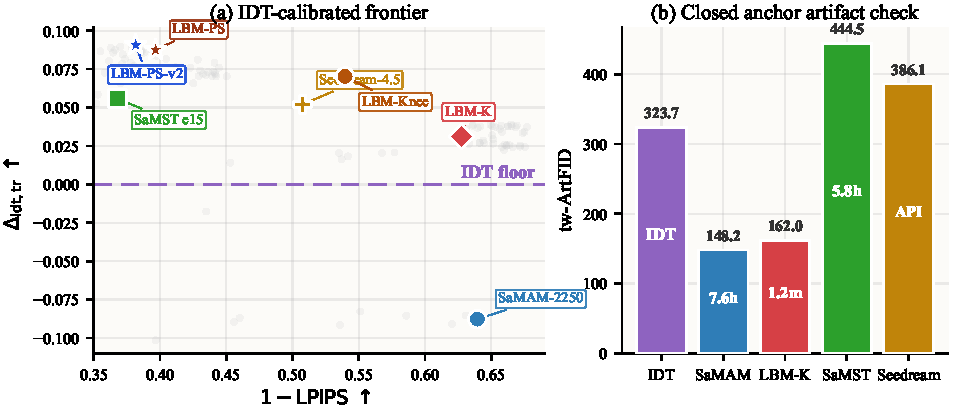
\includegraphics[width=0.965\textwidth]{figures/fig_distinct5_page1_summary.pdf}
\captionof{figure}{IDT-calibrated Distinct5-WikiArt summary under the shared packet. Panel (a) plots selected operating points in transfer-only $\Delta_{\mathrm{idt,tr}}$ versus $1-\mathrm{LPIPS}$ space, with faint gray dots showing the broader recorded development landscape. Conservative compact anchors remain near the low-damage regime, later successors move upward into a stronger style band, and Seedream-4.5 is shown as an external large-prior reference rather than a style-ID model. Panel (b) reports an all-pairs target-pooled ArtFID check for reproduced baselines, the selected LBM-Knee successor, and the Seedream reference.}
\label{fig:distinct5_page1}
\vspace{-5mm}
\end{strip}

\section{Introduction}
Domain-level artistic transfer asks a model to render a source image according to a target style identity rather than a target style exemplar. This setting exposes a simple but serious evaluation failure: when the source image is already artwork, the unchanged source can obtain high target-style affinity. A method may therefore appear competitive by preserving an art-domain prior, or by making visible but misdirected edits, without actually moving toward the requested target domain. We use the identical-image transfer (IDT) floor to make this failure explicit and report signed target-style movement above that floor.

Our target regime is also narrower and more practical than reference-guided or diffusion-prior stylization. At inference time, the model receives only a source image and a target style identifier; it should not require a style image, per-image optimization, or adaptation of a large generative prior. This makes the problem a low-cost customization problem as much as a stylization problem: the desired model should expose selectable style-content operating points while remaining compact enough to retrain on consumer hardware.

We propose \emph{Latent Bridge Matching} (LBM), a compact latent transport family in VAE space. In the current Distinct5 mainline, LBM combines training-side endpoint pairing, a style-conditioned latent field, and terminal SA-SWD with kinetic motion control. The resulting family forms a controllable IDT-calibrated frontier rather than a single conservative checkpoint: compact anchors clear the IDT floor in a low-damage regime, while StructOT and Pattern+Stokes successors move into a stronger high-style band under the same style-ID inference contract. This framing is what distinguishes the paper from both reference-guided stylization and large-prior adaptation lines \cite{gatys2016image,huang2017adain,liu2024samst,liu2025samam,zhang2024artbank,chung2024styleid,zhou2024comprehensiveeval,yeh2020calibrated,wright2022artfid}.

Our contributions are threefold.
\begin{itemize}
    \item \textbf{Evaluation diagnostic.} We introduce an IDT-calibrated protocol for domain-level art-to-art transfer, reporting transfer-only $\Delta_{\mathrm{IDT}}$ so that target-style movement is separated from the unchanged art-domain prior.
    \item \textbf{Method family.} We propose LBM, a compact style-ID latent transport family that separates training-side endpoint pairing, style-conditioned latent execution, kinetic motion control, and terminal SA-SWD matching in VAE space.
    \item \textbf{Frontier evidence.} We show that LBM is not a single conservative checkpoint but a controllable operating-point frontier on Distinct5-WikiArt: compact anchors clear the IDT floor at minute-scale training cost, the closed LBM-Knee point improves selected artifact/content diagnostics relative to the reproduced SaMST high-style baseline while remaining close on a held-out non-CLIP style probe, and two fixed-rule follow-up splits preserve the same IDT pathology beyond the main split.
\end{itemize}

\section{Related Work}
Arbitrary style transfer began with optimization-based feature reconstruction and Gram statistics \cite{gatys2016image}, then moved toward feed-forward alignment and local correspondence through AdaIN, SANet, ArtFlow, AdaAttN, StyTr2, and related variants \cite{huang2017adain,park2019sanet,an2021artflow,liu2021adaattn,deng2022stytr2}. More recent systems refine style injection through aesthetic guidance, semantic-region control, or stronger pretrained priors \cite{hong2023aespa,huang2024aesfa,zheng2024puffnet,zhang2025hsi,shang2025scsa,zhang2024artbank,chung2024styleid,deng2024zstar}. These methods mainly ask how a style exemplar or large prior should be used at inference. Our setting is different: inference receives only a target style identity, so the main question is whether a compact style-side representation remains executable after passing through a content-conditioned latent renderer.

The closest comparison line is efficient multi-style and compact style-ID transfer. SaMST studies style modeling and transfer through pluggable style representations \cite{liu2024samst}, while Mamba-ST and SaMam revisit global mixing through state-space backbones \cite{botti2025mambast,liu2025samam}. LBM contributes on the training and objective side: pairing-cache endpoint selection, compact latent transport, and terminal distribution matching under a style-ID interface. On the evaluation side, prior work already notes that automatic style-transfer metrics are inconsistent and can misalign with human judgment \cite{zhou2024comprehensiveeval,yeh2020calibrated,wright2022artfid}. This motivates our Distinct5 use of the unchanged-image floor and $\Delta_{\mathrm{idt}}$ as explicit diagnostics for whether a method actually moves toward the requested target style.

\section{Method}
\subsection{Overview}
LBM is a latent transport family in VAE space for domain-level artistic transfer. For the Distinct5-WikiArt packet, the source latent is $z_0 \in \mathbb{R}^{4 \times 64 \times 64}$; the historical CycleGAN-256 packet uses $4 \times 32 \times 32$ latents. Let $s$ denote a target style identifier. The active Distinct5 line combines four pieces: (i) training-side endpoint pairing that selects candidate target latents without paired supervision; (ii) a style-conditioned latent field that executes the requested motion; (iii) kinetic regularization that discourages unnecessary displacement; and (iv) terminal distribution matching that checks whether the resulting endpoint has target-style patch statistics. At inference, the model receives only the source image and target style identifier; target-domain latents remain training-side supervision only.

In the reproduced Distinct5 mainline, the active headline rows use endpoint-mode OMF training rather than the earlier random-time flow residual. Writing
\begin{equation}
    \hat v = v_\theta(z_0,1,s), \qquad \hat z_1 = z_0 + \hat v,
\end{equation}
the active objective is
\begin{equation}
    \mathcal{L}_{\mathrm{active}} =
    \lambda_{\mathrm{term}}\mathcal{L}_{\mathrm{term}}(\hat z_1)
    + \lambda_{\mathrm{kin}}\|\hat v\|_2^2,
    \label{eq:active_distinct5_loss}
\end{equation}
where candidate terminal targets are selected by the pairing cache and the parent flow residual is disabled in the headline rows ($w_{\mathrm{flow}}=0$). We therefore describe the paper-facing Distinct5 family as pairing-cache / terminal-SWD / kinetic OMF rather than as an online Sinkhorn or random-time flow-matching result family.

\begin{figure*}[t!]
    \centering
    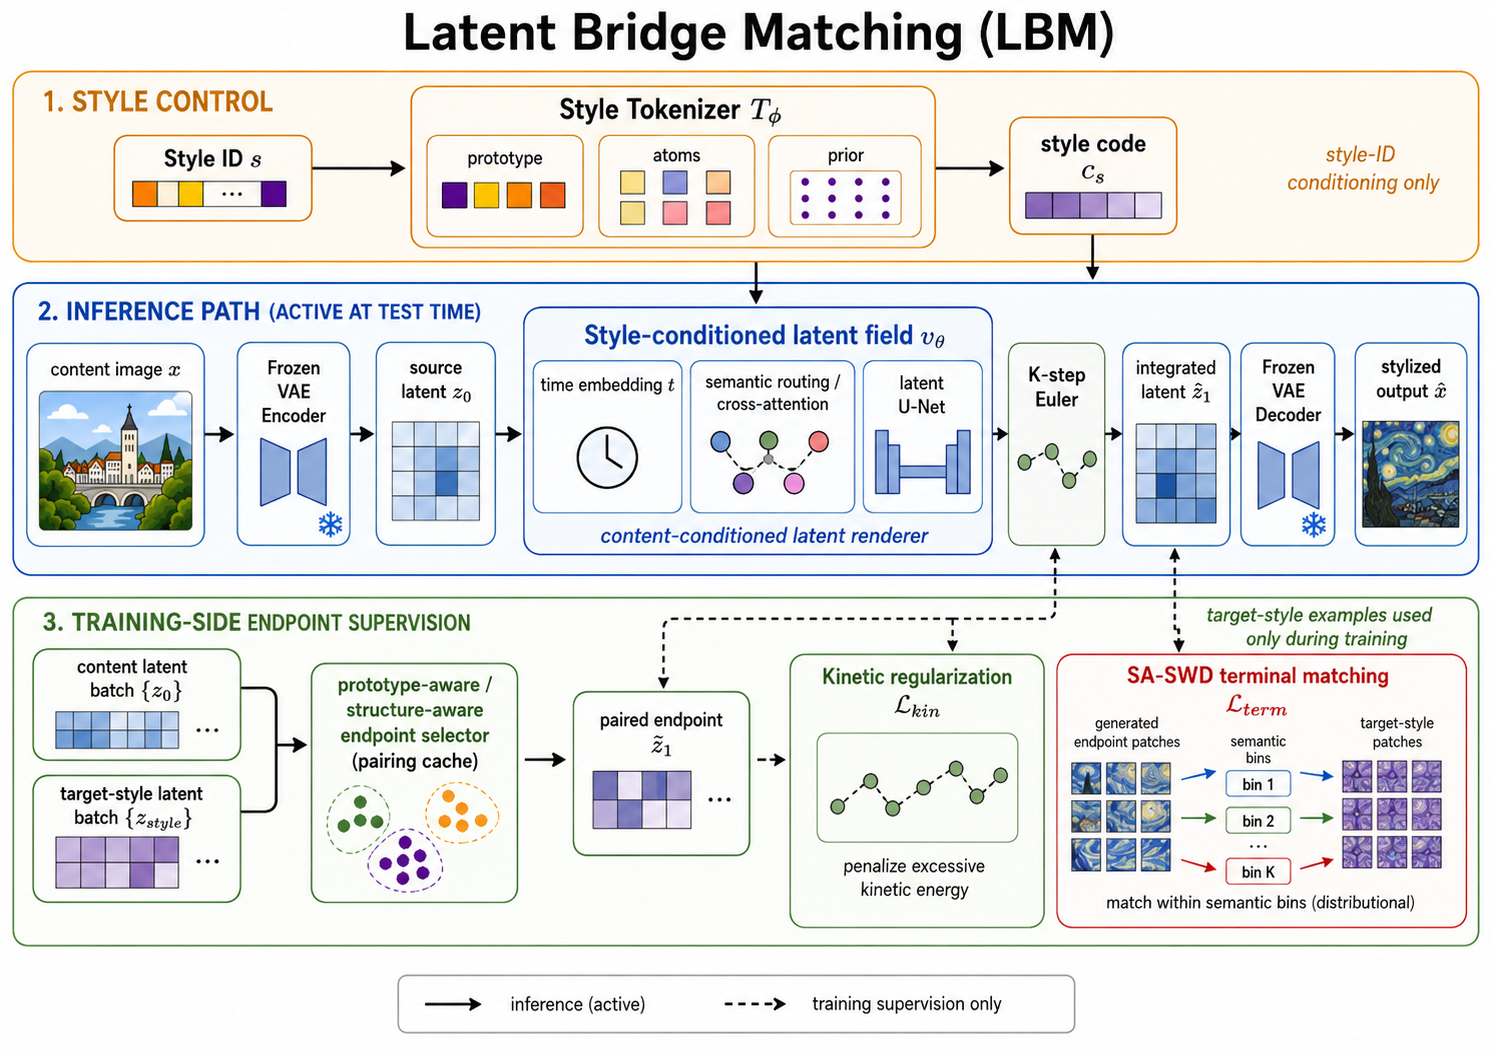
\includegraphics[width=0.86\textwidth]{framework_lbm_main_user.png}
    \caption{LBM combines a style tokenizer, a content-conditioned latent renderer, and training-side endpoint supervision with terminal SA-SWD.}
    \label{fig:framework}
\end{figure*}

\subsection{Endpoint pairing, execution, and terminal matching}
We train directly on precomputed VAE latents without paired supervision. For each source latent $z_0$ and target style $s$, the pairing cache exposes a selector-restricted candidate set $\mathcal{C}(z_0,s)$ from the target domain. The terminal target $\tilde z_1$ used by the loss is drawn from that scheduled set. This pairing step determines where supervision should pull, but not how much motion is actually executed.

Execution is handled by a time-conditioned latent backbone with sinusoidal time embeddings, style spatial priors, and semantic cross-attention. The style-side interface is separated from the renderer: the tokenizer receives only a target style identifier and produces a compact control code $c_s$, while the renderer decides how much latent motion is needed under the current content. In the current mainline this interface is paired with prototype-aware target queues and content-guided routing, which empirically improve executed style-content tradeoffs more reliably than simply enlarging the style code.

The endpoint is then regularized by semantic-aligned sliced Wasserstein distance. Let $\Phi_\theta(z_0,s)$ denote the Euler-integrated endpoint. The terminal objective is
\begin{equation}
    \mathcal{L}_{\mathrm{term}} =
    \mathrm{SWD}_1\bigl(\Phi_\theta(z_0,s),\,\tilde z_1\bigr),
\end{equation}
where sorted one-dimensional projections compare generated endpoint patches against target-style patches without requiring spatial correspondence. In the current SA-SWD instantiation, projection directions are chosen from the same routing signal that injects style into the backbone. This design keeps target-style pressure distributional rather than pointwise, which is important in compressed VAE latents where direct endpoint MSE encourages mean solutions. Bounded design-grounding analysis for kinetic regularization, Euler discretization, and the historical OT-style parent assignment map is retained as supplementary support rather than consuming main-paper space.

\paragraph{Operating-point variants.}
All reported LBM rows share the same style-ID inference contract: inference receives only the source image and target style identifier. LBM-K is the compact earlier-mainline anchor built from the content-adaptive tokenizer and queue curriculum used in the faster three-epoch packet, with active top-$2$ pairing and a $0.15$ queue-exploration probability over the top-$8$ candidate set, and with no explicit structure penalty. All promoted successor rows switch to an endpoint-prediction successor family with barycentric top-$8$ targets, low-frequency-plus-edge coupling, the manifold-adaptive kinetic split, and a cross-attention texture proximal branch. LBM-Knee adds joint anisotropic and Stokes transport control ($w_{\mathrm{aniso}}=1.0$, normal/tangent weights $25/0.25$, $w_{\mathrm{stokes}}=0.03$), together with queue-side dual-target smoothing (mix weight $0.5$) and auxiliary terminal SWD (weight $0.5$). LBM-PS keeps the same successor family but uses a higher Stokes coefficient, $w_{\mathrm{stokes}}=0.05$. LBM-PS-v2 changes one knob relative to LBM-PS, lowering the Stokes coefficient to $0.02$ to recover more style at the cost of higher LPIPS.

\section{Experiments}
\subsection{Protocol hierarchy and metrics}
We organize the evidence into two non-interchangeable result families, with Distinct5-WikiArt as the primary stress benchmark and the historical CycleGAN-256 packet as historical support. This separation is necessary because the same scalar pair, CLIP-style and LPIPS, can be misleading when datasets, image resolution, or baseline training protocols change.

\paragraph{Historical CycleGAN-256.}
The main legacy protocol uses five domains---photo, Hayao, Monet, Van Gogh, and Cezanne---and evaluates all $5\times5$ source-target directions with 30 source images per source domain, for 750 generated outputs. This is the protocol used for comparisons to SaMST, S2WAT, StyleID, AdaIN, StyTr2, CAST, AesFA, and AesPA-Net.

\paragraph{Distinct5-WikiArt stress split.}
The new stress split uses Early Renaissance, Impressionism, Minimalism, Rococo, and Ukiyo-e, with 1000 training images and 30 held-out test images per class. These five classes were chosen as the most strongly separated subset under a CLIP-style screening pass over WikiArt categories, rather than being hand-picked for LBM. Evaluation again uses all $5\times5$ directions over 750 generated images. This split complements the historical table with a stronger domain-separation test and an explicit identical-image baseline.

We report CLIP-style (CLIP-S) and CLIP-content (CLIP-C) using CLIP ViT-B/32 embeddings \cite{radford2021clip}, together with LPIPS-content and
\begin{equation}
    \mathrm{EC} = \mathrm{CLIP\mbox{-}style}\cdot(1-\mathrm{LPIPS}).
\end{equation}
For Distinct5-WikiArt we additionally report style gain over the unchanged-image reference,
\begin{equation}
    \Delta_{\mathrm{idt}} = \mathrm{CLIP\mbox{-}S}(\text{method}) - \mathrm{CLIP\mbox{-}S}(\text{idt}),
\end{equation}
under both the full 5$\times$5 protocol and the transfer-only off-diagonal subset. We use this quantity to define the metric-stress regime exposed by Distinct5-WikiArt: raw CLIP-style should not be treated as sufficient evidence of successful target-style transfer if a method either fails to exceed the identical-image prior ($\Delta_{\mathrm{idt}}\le 0$) or exceeds it only by moving into a clearly damaged LPIPS region while also deteriorating broad artifact diagnostics. In this paper, CLIP-S is interpreted as target-style affinity, LPIPS as content displacement, and targetwise ArtFID as a target-domain plausibility and artifact diagnostic rather than a direct style-gain score. Aggregate ArtFID is kept only as an auxiliary art-domain/identity diagnostic outside this main Distinct5 comparison. In particular, lower targetwise ArtFID alone does not certify useful stylization on separated art-to-art transfer: its content term rewards source preservation, and its distributional term can reward remaining in a plausible target-domain art manifold even when the requested target-style movement is still below the unchanged-image baseline. EC is used only as a Pareto summary; claims are checked against CLIP-S and LPIPS individually. For artifact-sensitive analysis we also report MUSIQ, MANIQA, DISTS-content, high-frequency patch KID, FFT slope error, shallow Gram micro statistics, and KID where available. All CycleGAN-256 baselines use the same source images, target domains, preprocessing, and identity directions. For arbitrary-style methods, one target-domain reference image is supplied per target style; for style-id LBM, the model receives only the target domain identifier. The `idt' control is introduced here as a split-specific diagnostic baseline for art-to-art transfer: Distinct5-WikiArt makes the unchanged-image prior explicit on this split.

\subsection{Distinct5-WikiArt stress benchmark}
Distinct5-WikiArt is an IDT-calibrated operating-point benchmark, not a single-score leaderboard. All five domains come from standard WikiArt classes and are selected because they are strongly separated under a CLIP-style screening pass. In this regime, unchanged output is no longer a plausible success proxy: the \emph{idt} baseline already reaches CLIP-S 0.6801 while doing no transfer at all. Signed target-style movement is therefore the first sanity check. Under the shared full 5$\times$5 / 750-output protocol, the earlier compact anchors LBM-F/K establish a conservative low-damage regime: LBM-F reaches transfer CLIP-S 0.6644 with LPIPS 0.3245 after 1.2 minutes of checkpoint training, and LBM-K raises style to 0.6712 at LPIPS 0.3723 while remaining well below the SaMST damage band. The more important result is that the family does not stop there. A promoted content-preserving successor now reaches 0.7102 transfer CLIP-S at 0.5397 content preservation $(1-\mathrm{LPIPS})$, while the higher-style successors push the frontier to 0.7274 / 0.3967 and 0.7307 / 0.3817 in transfer CLIP-S / $(1-\mathrm{LPIPS})$. This is a family-level frontier with three practically different regimes: conservative low-damage anchors, a content-preserving successor knee, and a style-ceiling operating point.

We fix representative rows before qualitative inspection. The manuscript table reports one compact anchor from the earlier mainline, one lower-LPIPS successor tradeoff point, one balanced high-style point, and one style-ceiling point. The broader development landscape is shown only as faint background support in Figure~\ref{fig:distinct5_page1}, not as a second leaderboard.

The reproduced baselines remain important because they bound those regimes. SaMST e15 reaches 0.6957 / 0.6319 and can produce locally strong target-style jumps, but it does so in a clearly higher-damage region and with targetwise ArtFID 395.7 on the full scope and 444.5 on the transfer-only scope; the retained e5/e15 packet is already near a plateau on transfer CLIP-S and LPIPS, with less than 0.004 / 0.002 difference between the checkpoints. Seedream-4.5 provides a stronger external large-prior reference under a fixed API protocol: we use the source image together with a fixed target-domain prompt template of the form ``convert the image to \textit{<style>} style,'' without retraining or style-ID control. Its transfer row is 0.6920 / 0.4923, which is better than the compact anchor but still below the promoted LBM knee point on both style gain and content preservation. At the same time, Seedream keeps the strongest identity row among the currently compared points, which is why we treat it as a useful outer reference rather than as a same-interface baseline. At the trusted SaMAM 2250 checkpoint, transfer CLIP-S remains below the IDT floor even though targetwise ArtFID improves to 146.1 on the full scope and 148.2 on the transfer-only scope. This is the evaluation failure exposed by Distinct5: lower targetwise ArtFID can still coincide with zero or negative target-style gain when a method preserves source structure and stays inside a plausible target-art manifold without moving toward the requested target style. Distinct5 therefore turns the paper's evaluation claim into an operating-point test within this split: target-style movement should be demonstrated relative to IDT, and a paper-facing result should be reported as a selected Pareto point rather than as one arbitrarily chosen checkpoint.

\begin{table}[t]
\centering
\caption{Selected Distinct5-WikiArt operating points under the shared transfer-only packet. `idt' is the unchanged-image floor. Rows are chosen to represent distinct roles on the current frontier rather than a single checkpoint family: a compact conservative anchor, a content-preserving successor knee, two higher-style promoted successors, and one external large-prior reference. We report only transfer-scope metrics here so the main table does not mix all-pairs and transfer-only readings.}
\label{tab:distinct5}
\small
\setlength{\tabcolsep}{3.5pt}
\resizebox{\columnwidth}{!}{%
\begin{tabular}{@{}l l r r r l@{}}
\toprule
Point & Role & CLIP-S$_{\mathrm{tr}}\uparrow$ & $1-\mathrm{LPIPS}\uparrow$ & $\Delta_{\mathrm{idt,tr}}\uparrow$ & Closure \\
\midrule
idt & no-op floor & 0.6399 & 1.0000 & 0.0000 & closed \\
SaMAM-2250 & compact baseline & 0.5523 & 0.6395 & -0.0877 & closed \\
SaMST e15 & high-style baseline & 0.6957 & 0.3681 & +0.0558 & closed \\
Seedream-4.5 & large-prior ref. & 0.6920 & 0.5077 & +0.0521 & closed \\
LBM-K e1 & conservative anchor & 0.6712 & 0.6277 & +0.0312 & closed \\
LBM-Knee e13 & content-preserving successor & 0.7102 & \textbf{0.5397} & +0.0703 & closed \\
LBM-PS e13 & balanced high-style & 0.7274 & 0.3967 & +0.0875 & frontier \\
LBM-PS-v2 e13 & style ceiling & \textbf{0.7307} & 0.3817 & \textbf{+0.0908} & frontier \\
\bottomrule
\end{tabular}
}
\end{table}

Table~\ref{tab:cost_distinct5} isolates the recorded operating-point cost under the same Distinct5 packet, but only for rows whose timing provenance is already fully closed. The broader successor family should therefore be read as a quality frontier first, not as a normalized timing leaderboard: the later Pattern+Stokes and structure-aware OT packets strengthen the style side of the frontier, while compact-anchor timing remains the cleanest accessibility evidence. The qualitative interpretation is consistent with the table-level result: SaMST can produce locally strong target-style jumps, but those gains sit in a much higher-damage region, Seedream-4.5 remains an out-of-interface large-prior reference rather than a style-ID baseline, and SaMAM still often edits without producing reliable target-style movement above the no-op floor.

The same reading survives an explicit three-scope check on the promoted content-preserving successor. A local retest of the selected e13 knee point gives transfer 0.7101 / 0.4604, all-pairs 0.7302 / 0.4560, and identity 0.8105 / 0.4384 in CLIP-S / LPIPS. Its all-pairs targetwise ArtFID is 388.2 under the same target-pooled protocol used for the page-1 artifact panel. For context, Seedream-4.5 gives transfer 0.6920 / 0.4923, all-pairs 0.7198 / 0.4767, identity 0.8312 / 0.4145, and all-pairs targetwise ArtFID 311.5 under the same repaired-750 target-pooled recompute. The promoted LBM successor therefore improves target-style movement and content preservation over this large-prior reference on the transfer and all-pairs scopes, while Seedream keeps the strongest identity row and lower all-pairs ArtFID. Seedream is not a same-interface baseline; it is an external large-prior reference.

\begin{table}[t]
\centering
\caption{Auxiliary artifact-sensitive and non-CLIP diagnostics on selected Distinct5-WikiArt rows. tw-ArtFID uses the all-pairs target-pooled recompute; Gram-$\mu$ is a shallow VGG Gram distance; EdgePurity is a higher-is-better content-edge diagnostic; NonCLIPAcc is the transfer-only target accuracy from the held-out ConvNeXt style probe.}
\label{tab:distinct5_artifact_aux}
\small
\setlength{\tabcolsep}{3.4pt}
\resizebox{\columnwidth}{!}{%
\begin{tabular}{@{}l r r r r@{}}
\toprule
Point & tw-ArtFID$_{\mathrm{all}}\downarrow$ & Gram-$\mu\downarrow$ & EdgePurity$\uparrow$ & NonCLIPAcc$\uparrow$ \\
\midrule
LBM-K e1 & 316.5 & 0.153 & \textbf{0.540} & 0.167 \\
LBM-Knee e13 & 388.2 & \textbf{0.137} & 0.288 & 0.237 \\
LBM-PS-v2 e13 & 465.6 & 0.183 & 0.115 & 0.272 \\
SaMST e15 & 395.7 & 0.147 & 0.102 & 0.248 \\
Seedream-4.5 & \textbf{311.5} & 0.189 & 0.389 & \textbf{0.378} \\
\bottomrule
\end{tabular}
}
\end{table}

Table~\ref{tab:distinct5_artifact_aux} sharpens the role split inside the frontier. Relative to SaMST e15, the selected Knee point lowers all-pairs target-pooled ArtFID (388.2 vs.\ 395.7), improves shallow texture statistics (Gram-$\mu$ 0.137 vs.\ 0.147), and more than doubles the edge-purity diagnostic (0.288 vs.\ 0.102). A held-out ConvNeXt-Tiny probe trained on the 5,000-image Distinct5 train split reaches 96\% accuracy on the 150-image test split; on transfer-only outputs it assigns target accuracy 1.0\% to IDT, 16.7\% to LBM-K, 23.7\% to LBM-Knee, 24.8\% to SaMST, 27.2\% to PS-v2, and 37.8\% to Seedream. Knee and SaMST are therefore close on non-CLIP target recognition, but Knee is substantially cleaner on artifact diagnostics. Row-resampled transfer bootstrap also keeps both promoted rows strictly above IDT: Knee $\Delta_{\mathrm{idt,tr}}=0.0702$ with $[0.0635, 0.0769]$, and PS-v2 $\Delta_{\mathrm{idt,tr}}=0.0901$ with $[0.0826, 0.0976]$. We therefore treat LBM-Knee as the main closed Pareto point and keep PS-v2 as the explicit style-ceiling row rather than a universal winner.

\begin{figure*}[t]
    \centering
    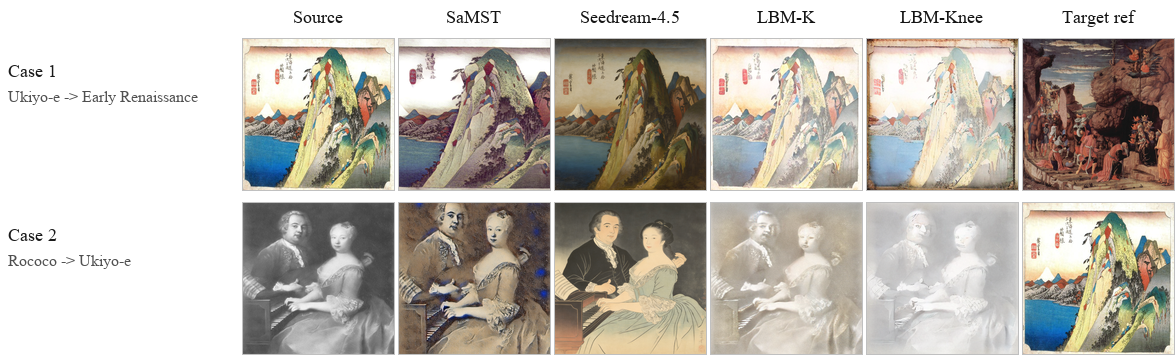
\includegraphics[width=0.985\textwidth]{figures/fig_distinct5_qualitative_main.png}
    \caption{Main-paper qualitative comparison on Distinct5-WikiArt. Columns show `Source | SaMST | Seedream-4.5 | LBM-K | LBM-Knee | target-domain ref'. Target-domain references are shown only for visualization and are not provided to LBM at inference. The top row highlights the main Pareto tradeoff on a Ukiyo-e $\rightarrow$ Early Renaissance transfer: the reproduced compact baseline moves more aggressively, while LBM-Knee keeps a more conservative structure-preserving rendering than the stronger style references. The bottom row shows the same contrast on a Rococo $\rightarrow$ Ukiyo-e transfer. The stronger style-ceiling PS-v2 row and the aligned SaMAM-2250 negatives are kept in the supplement, where they read more naturally as supporting comparisons than as the main visual headline.}
    \label{fig:qual_main}
\end{figure*}

Figure~\ref{fig:qual_main} shows why the frontier interpretation is more informative than a single checkpoint claim. In both cases, SaMST and Seedream move farther toward the target style, but they also pay more heavily in structure preservation. LBM-K remains the most conservative moving point, while LBM-Knee keeps much more of the source layout than the stronger style references and still moves past the compact anchor.

% Evidence-backed timing tables for direct use via:
% % Evidence-backed timing tables for direct use via:
% % Evidence-backed timing tables for direct use via:
% \input{snippets/timing_tables_leibniz}
% ...
% \HistoricalTimingTableLeibniz
% ...
% \DistinctFiveTimingTableLeibniz

\newcommand{\HistoricalTimingTableLeibniz}{%
\begin{table}[t]
\centering
\footnotesize
\setlength{\tabcolsep}{4pt}
\caption{Historical strict-750 / 256$\times$256 recorded operating-point cost. Training time is the wall-clock cost to the manuscript operating point; inference is the end-to-end runtime for the 750-image protocol. This is recorded operating-point context, not a normalized time-to-quality comparison.}
\label{tab:cost}
\begin{tabular}{@{}lccc@{}}
\toprule
Method & Train to point & Infer-750 & ms/img \\
\midrule
LBM & \textbf{5.2 min} & 85.4 s & 114 \\
\bottomrule
\end{tabular}

\vspace{2pt}
\parbox{0.98\linewidth}{\raggedright\footnotesize\textit{Note.} The LBM row is a preserved timing record. Other historical rows are intentionally omitted here because the available train/infer evidence is either probe-estimated, mixed-protocol, or incomplete rather than a closed operating-point packet.}
\end{table}%
}

\newcommand{\DistinctFiveTimingTableLeibniz}{%
\begin{table}[t]
\centering
\footnotesize
\setlength{\tabcolsep}{4pt}
\caption{Distinct5-512 recorded operating-point cost under the reviewed full $5\times5$ / 750-output packet. Reported train time is cumulative training wall-clock to the shown checkpoint, with evaluation excluded. This is recorded operating-point cost, not a normalized time-to-quality comparison.}
\label{tab:cost_distinct5}
\begin{tabular}{@{}lcc@{}}
\toprule
Method & Recorded point & Train to point \\
\midrule
LBM-F & e1 & \textbf{1.2 min} \\
LBM-K & e1 & \textbf{1.2 min} \\
SaMAM & step 2250 & 7.6 h \\
SaMST & e15 & 5.8 h \\
\bottomrule
\end{tabular}

\vspace{2pt}
\parbox{0.98\linewidth}{\raggedright\footnotesize\textit{Note.} Distinct5 times are cumulative training wall only, with evaluation excluded. We intentionally omit a shared inference column because same-grade pure-generation timing is still incomplete for the active manuscript rows \texttt{SaMAM-2250} and \texttt{SaMST-e15}; leaving blanks would overstate closure. Post-2250 SaMAM timings are intentionally excluded.}
\end{table}%
}

% ...
% \HistoricalTimingTableLeibniz
% ...
% \DistinctFiveTimingTableLeibniz

\newcommand{\HistoricalTimingTableLeibniz}{%
\begin{table}[t]
\centering
\footnotesize
\setlength{\tabcolsep}{4pt}
\caption{Historical strict-750 / 256$\times$256 recorded operating-point cost. Training time is the wall-clock cost to the manuscript operating point; inference is the end-to-end runtime for the 750-image protocol. This is recorded operating-point context, not a normalized time-to-quality comparison.}
\label{tab:cost}
\begin{tabular}{@{}lccc@{}}
\toprule
Method & Train to point & Infer-750 & ms/img \\
\midrule
LBM & \textbf{5.2 min} & 85.4 s & 114 \\
\bottomrule
\end{tabular}

\vspace{2pt}
\parbox{0.98\linewidth}{\raggedright\footnotesize\textit{Note.} The LBM row is a preserved timing record. Other historical rows are intentionally omitted here because the available train/infer evidence is either probe-estimated, mixed-protocol, or incomplete rather than a closed operating-point packet.}
\end{table}%
}

\newcommand{\DistinctFiveTimingTableLeibniz}{%
\begin{table}[t]
\centering
\footnotesize
\setlength{\tabcolsep}{4pt}
\caption{Distinct5-512 recorded operating-point cost under the reviewed full $5\times5$ / 750-output packet. Reported train time is cumulative training wall-clock to the shown checkpoint, with evaluation excluded. This is recorded operating-point cost, not a normalized time-to-quality comparison.}
\label{tab:cost_distinct5}
\begin{tabular}{@{}lcc@{}}
\toprule
Method & Recorded point & Train to point \\
\midrule
LBM-F & e1 & \textbf{1.2 min} \\
LBM-K & e1 & \textbf{1.2 min} \\
SaMAM & step 2250 & 7.6 h \\
SaMST & e15 & 5.8 h \\
\bottomrule
\end{tabular}

\vspace{2pt}
\parbox{0.98\linewidth}{\raggedright\footnotesize\textit{Note.} Distinct5 times are cumulative training wall only, with evaluation excluded. We intentionally omit a shared inference column because same-grade pure-generation timing is still incomplete for the active manuscript rows \texttt{SaMAM-2250} and \texttt{SaMST-e15}; leaving blanks would overstate closure. Post-2250 SaMAM timings are intentionally excluded.}
\end{table}%
}

% ...
% \HistoricalTimingTableLeibniz
% ...
% \DistinctFiveTimingTableLeibniz

\newcommand{\HistoricalTimingTableLeibniz}{%
\begin{table}[t]
\centering
\footnotesize
\setlength{\tabcolsep}{4pt}
\caption{Historical strict-750 / 256$\times$256 recorded operating-point cost. Training time is the wall-clock cost to the manuscript operating point; inference is the end-to-end runtime for the 750-image protocol. This is recorded operating-point context, not a normalized time-to-quality comparison.}
\label{tab:cost}
\begin{tabular}{@{}lccc@{}}
\toprule
Method & Train to point & Infer-750 & ms/img \\
\midrule
LBM & \textbf{5.2 min} & 85.4 s & 114 \\
\bottomrule
\end{tabular}

\vspace{2pt}
\parbox{0.98\linewidth}{\raggedright\footnotesize\textit{Note.} The LBM row is a preserved timing record. Other historical rows are intentionally omitted here because the available train/infer evidence is either probe-estimated, mixed-protocol, or incomplete rather than a closed operating-point packet.}
\end{table}%
}

\newcommand{\DistinctFiveTimingTableLeibniz}{%
\begin{table}[t]
\centering
\footnotesize
\setlength{\tabcolsep}{4pt}
\caption{Distinct5-512 recorded operating-point cost under the reviewed full $5\times5$ / 750-output packet. Reported train time is cumulative training wall-clock to the shown checkpoint, with evaluation excluded. This is recorded operating-point cost, not a normalized time-to-quality comparison.}
\label{tab:cost_distinct5}
\begin{tabular}{@{}lcc@{}}
\toprule
Method & Recorded point & Train to point \\
\midrule
LBM-F & e1 & \textbf{1.2 min} \\
LBM-K & e1 & \textbf{1.2 min} \\
SaMAM & step 2250 & 7.6 h \\
SaMST & e15 & 5.8 h \\
\bottomrule
\end{tabular}

\vspace{2pt}
\parbox{0.98\linewidth}{\raggedright\footnotesize\textit{Note.} Distinct5 times are cumulative training wall only, with evaluation excluded. We intentionally omit a shared inference column because same-grade pure-generation timing is still incomplete for the active manuscript rows \texttt{SaMAM-2250} and \texttt{SaMST-e15}; leaving blanks would overstate closure. Post-2250 SaMAM timings are intentionally excluded.}
\end{table}%
}

\DistinctFiveTimingTableLeibniz

\paragraph{Adaptation cost and accessibility.}
Figure~\ref{fig:distinct5_page1} makes the practical gap visible without resorting to a synthetic normalized speedup claim. Conservative LBM anchors cross the Distinct5-WikiArt IDT floor after 1.2 minutes of training on a single RTX 3060, whereas the trusted SaMAM-2250 checkpoint remains below that floor after 7.6 hours and SaMST exceeds it only after 5.8 hours in a much higher-damage region. Within this domain-style setting, compact latent transport shifts customized stylization from a resource-intensive adaptation problem toward a minute-scale small-model learning problem.

\subsection{Historical support and secondary evidence}
We keep the historical CycleGAN-256 packet as historical support rather than as a second main benchmark. On that older surface, LBM remains a competitive compact retrainable point with 0.7161 CLIP-S / 0.4514 LPIPS at 114\,ms/image, while the strongest reproduced competing rows either collapse content or enter noisier artifact regimes. Two fixed-rule follow-up WikiArt stress splits also preserve the main evaluator pattern: on split1 and split2, unchanged images still score strongly, and compact LBM-F remains above the split-local IDT floor by `+0.0139` and `+0.0073` transfer CLIP-S respectively. The same policy applies to ablations: content-guided execution and prototype-aware target queues improve the frontier more reliably than larger undifferentiated style codes, and terminal distribution matching remains the primary style driver. All reported evaluations use fixed seeds, stored resolved configurations, source snapshots, checkpoints, and per-epoch logs. Historical timings were measured on an RTX 4070 Laptop GPU unless otherwise noted. The supplement lists the artifact ledger, Seedream protocol, target-pooled ArtFID recompute path, the fixed-rule split packets, and the non-CLIP style probe.



\section{Discussion and Limitations}
The main lesson is that style transfer quality cannot be inferred from raw CLIP-style alone. Distinct5-WikiArt sharpens this point because the no-op baseline is measured explicitly: some baselines fail even to exceed the identical-image prior, while others exceed it only by moving into severe LPIPS and targetwise ArtFID failure regions. This exposes a practical blind spot in art-to-art evaluation: preserved art-domain priors can masquerade as target-style success unless the unchanged-image floor is reported \cite{zhou2024comprehensiveeval,yeh2020calibrated,wright2022artfid}. These results also change the role of LBM from a single operating point to a selectable style-content family. Conservative anchors occupy the low-damage regime, LBM-Knee becomes the main closed Pareto point, and later Pattern+Stokes successors define the style ceiling. The practical consequence is that meaningful style-id customization can remain a small-model learning problem rather than a large-prior adaptation problem.

The tokenizer experiments narrow the remaining mechanism question. Raw code capacity alone is not the bottleneck; the harder issue is whether target-style information survives execution through a content-conditioned vector field strongly enough to yield real style gain beyond the unchanged-image reference. The current evidence therefore favors target-style carriers, prototype-aware queues, and content-aware routing over undifferentiated token expansion.

The study has several limitations. First, the main protocol is domain-level rather than reference-image-specific, so it does not attempt to reproduce a unique style image. Second, Euler integration is deliberately simple; although the step sweep is stable in the reported regime, more aggressive paths or higher resolutions may need better solvers or stronger constraints. Third, SA-SWD is an adaptive-projection distribution loss; current controls show that most of its benefit comes from the distributional term rather than from the specific semantic projection rule. Fourth, artifact-sensitive metrics are still proxies for visual preference; human studies or rubric-based VLM assessment would strengthen the claim further. In particular, the content-preserving successor now has transfer-style, LPIPS, targetwise ArtFID, non-CLIP probe, and qualitative closure, whereas the stronger style-ceiling rows still lack full human-preference closure. Finally, Distinct5-WikiArt is a five-domain stress split rather than a universal art benchmark, so broader domain coverage remains future work even though the current fixed-rule follow-up splits already show that the unchanged-image pathology is not unique to one class set.

\section{Conclusion}
We presented Latent Bridge Matching, a compact latent transport design for domain-level artistic transfer. The method separates training-side endpoint selection, path-wise field learning, adaptive-projection terminal distribution matching, and style-tokenized execution. Under the reproduced historical CycleGAN-256 protocol, LBM delivers a favorable reproduced balance of style strength, content fidelity, artifact control, and practical footprint within the mixed-family comparison packet considered here. The Distinct5-WikiArt stress benchmark sharpens the paper's main evaluation point: once the identical-image prior is made explicit, target-style movement must be read against IDT rather than from raw CLIP-S or ArtFID alone. On that split, LBM is a controllable family of operating points: conservative compact anchors clear the IDT floor early, LBM-Knee is the main closed Pareto point under artifact-sensitive and non-CLIP checks, and later Pattern+Stokes successors move into a stronger high-style regime.

Just as importantly, the reproduced minute-scale RTX 3060 adaptation path and the 3.91M / 114\,ms historical operating point show that customized stylization can remain a small-model learning problem rather than a large-prior adaptation problem, lowering the barrier for researchers and creators who want low-cost style-specific models on consumer GPUs. The tokenizer study then isolates the remaining mechanism question. Within the tested Distinct5 tokenizer variants, matched localization controls show that executor-side refresh recovers more than style-side refresh alone on the current local surface, while the same-family H path-stability packet indicates that kinetic regularization acts as a practical stabilizer in the current OMF / field regime. The next representation target is therefore to preserve target-style separation through execution itself, via explicit target carriers and tighter content-risk control.

\bibliography{refs}

\small
\setlength{\itemsep}{1pt}
\setlength{\parskip}{2pt}
\section*{Reproducibility Checklist}
\noindent\textbf{This paper}
\begin{itemize}
\item Includes a conceptual outline and/or pseudocode description of AI methods introduced: \textbf{Yes}.
\item Clearly delineates statements that are opinions, hypothesis, and speculation from objective facts and results: \textbf{Yes}.
\item Provides well marked pedagogical references for less-familiar readers to gain background necessary to replicate the paper: \textbf{Yes}.
\end{itemize}

\noindent\textbf{Does this paper make theoretical contributions?} \textbf{Yes (design-grounding)}. The paper provides compact formal analysis with proofs and empirical checks: Theorem~1 and Theorem~2 analyze the active field/solver regime through a path-action decomposition for kinetic regularization and an $O(1/K)$ Euler discretization bound, while Theorem~3 analyzes a historical OT-style assignment variant as family-level background. Full proofs are in the supplement. These results justify the three-part design without asserting equivalence to a full Schr\"odinger Bridge solver.

\noindent\textbf{Does this paper rely on one or more datasets?} \textbf{Yes}.
\begin{itemize}
\item A motivation is given for why the experiments are conducted on the selected datasets: \textbf{Yes}.
\item All novel datasets introduced in this paper are included in a data appendix: \textbf{NA}.
\item All novel datasets introduced in this paper will be made publicly available upon publication of the paper with a license that allows free usage for research purposes: \textbf{NA}.
\item All datasets drawn from the existing literature are accompanied by appropriate citations: \textbf{Yes}.
\item All datasets drawn from the existing literature are publicly available: \textbf{Yes}.
\item All datasets that are not publicly available are described in detail, with explanation why publicly available alternatives are not scientifically satisficing: \textbf{NA}.
\end{itemize}

\noindent\textbf{Does this paper include computational experiments?} \textbf{Yes}.
\begin{itemize}
\item This paper states the number and range of values tried per (hyper-)parameter during development of the paper, along with the criterion used for selecting the final parameter setting: \textbf{Partial}.
\item Any code required for pre-processing data is included in the appendix: \textbf{Partial} (the supplement lists the reviewed script paths and artifact roots for the current paper-facing packets).
\item All source code required for conducting and analyzing the experiments is included in a code appendix: \textbf{Partial} (the supplement enumerates the main reviewed scripts, configs, and eval artifacts, but does not inline the full codebase).
\item All source code required for conducting and analyzing the experiments will be made publicly available upon publication of the paper with a license that allows free usage for research purposes: \textbf{Partial}.
\item All source code implementing new methods have comments detailing the implementation, with references to the paper where each step comes from: \textbf{Partial}.
\item If an algorithm depends on randomness, then the method used for setting seeds is described in a way sufficient to allow replication of results: \textbf{Partial} (the supplement records the reviewed seed settings for the current paper-facing packets, but external references such as Seedream do not expose a user-controlled seed).
\item This paper specifies the computing infrastructure used for running experiments, including hardware/software details: \textbf{Yes}.
\item This paper formally describes evaluation metrics used and explains the motivation for choosing these metrics: \textbf{Yes}.
\item This paper states the number of algorithm runs used to compute each reported result: \textbf{Yes}.
\item Analysis of experiments goes beyond single-dimensional summaries of performance to include measures of variation, confidence, or other distributional information: \textbf{Yes}.
\item The significance of any improvement or decrease in performance is judged using appropriate statistical tests: \textbf{Partial} (selected confidence intervals and bootstrap summaries are reported, but not every manuscript comparison is presented as a closed significance claim).
\item This paper lists all final (hyper-)parameters used for each model/algorithm in the paper's experiments: \textbf{Partial}.
\end{itemize}

\end{document}



